\section{Research Decisions Behind the Main Narrative}
\label{app:narrative-support}

The article's main text now follows one question: which physical intervention explains a sparse PMU history, and when is that explanation distinguishable? The supporting studies below retain different estimators and denominators. They are evidence for particular steps in that argument, not a pooled test of a completed joint estimator.

\begin{table*}[t]\centering\small
\caption{Exploration changes the next inference question, not the test labels.}\label{tab:supp-research-decisions}
\begin{tabularx}{\textwidth}{@{}lXXX@{}}\toprule
Question explored & Observation & Decision retained & Boundary\\\midrule
Can eight PMUs constrain hidden voltage? & Accurate matched reconstruction; shift degrades it & Keep the physical state and operating context explicit & State recovery is not source attribution\\
Can an offset repair all mismatch? & Hidden-state recovery needs AC-feasible recentering & Separate physical recentering from measured residual centering & R11 intercept is not a new hidden-state solution\\
Does a source label transfer? & Legacy held-source test fails & Generate physical hypotheses for candidate assets & Causal unseen-source transfer remains untested\\
Does detecting multiplicity locate both sources? & Weak exact supports overlap & Profile severity/nuisance and keep alternatives & Batch onset/family known\\
Does every plausible multi-family proposal become a correct final decision? & The exploratory pilot does not establish that & Keep E\_J as proposed, not a validated replacement for E\_B & Dossier-only results remain secondary\\
Can a frozen physical bank follow successive events? & H04 separates timely recognition from eventual attribution & Retain dynamic recovery and compare nominal/mixture & Development, known catalog\\
Can stricter episode admission remove extras for free? & It rejects a real BUS16 intervention & Keep the failed ablation and freeze co-references & Zero extras is not uniform improvement\\
Does the result persist under an independent draw? & C01 is prespecified & No further method selection on that examination & Results enter only after complete evaluation\\\bottomrule
\end{tabularx}\end{table*}

\subsection{Connection to the Current Causal Method}
The complete local amplitude derivation and conditional-state update now
appear in Appendix~\ref{app:causal-calculations}, with worked examples.
They describe the causal history bank, not the batch estimator's GH31
quadrature. The remaining evidence in this appendix preserves the earlier
state-recovery and source-resolution contracts.

\subsection{State Recovery and Model Adequacy}
The matched B2 mean hidden-voltage error is \BTwoTVE{}, compared with \BZeroTVE{} for the equilibrium reference. Under the tested operating shifts, frozen errors of \EZeroHFrozenHalf{}, \EZeroHFrozenOne{} and \EZeroHFrozenMax{} become \EZeroHCorrectedHalf{}, \EZeroHCorrectedOne{} and \EZeroHCorrectedMax{} after regularized physical recentering. The nuisance information rank is \EZeroHRank{} of \EZeroHDimension{}. This supports a useful point target while leaving parameter non-uniqueness and joint covariance failure visible.

\begin{figure*}[t]\centering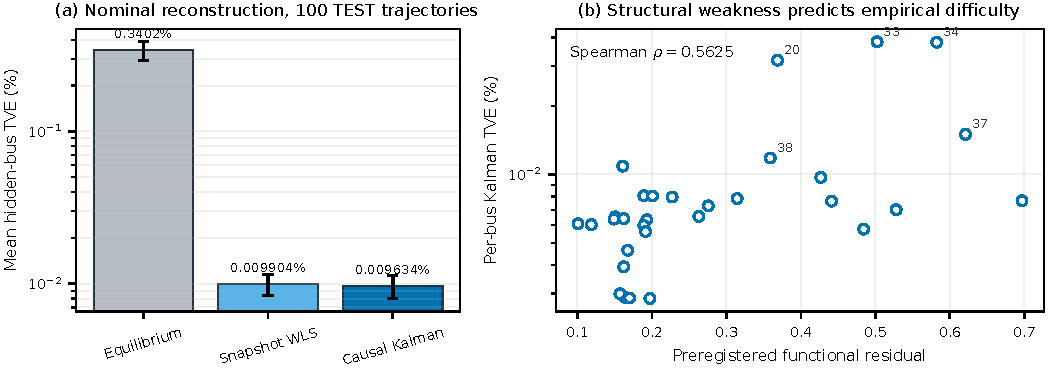
\includegraphics[width=\textwidth]{figures/generated/nominal_reconstruction.pdf}
\caption{Expanded matched state evidence, retained from the original frozen study. It evaluates hidden-voltage reconstruction and does not certify source identity.}\label{fig:supp-narrative-state}\end{figure*}
\begin{figure*}[t]\centering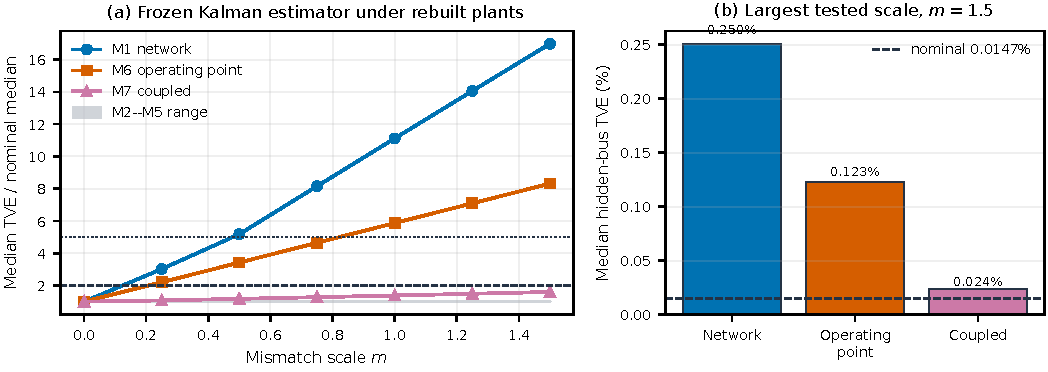
\includegraphics[width=\textwidth]{figures/generated/physical_mismatch.pdf}
\caption{Expanded model-mismatch evidence. Physical and operating shifts are distinct from instrumental covariance corrections.}\label{fig:supp-narrative-mismatch}\end{figure*}
\begin{figure*}[t]\centering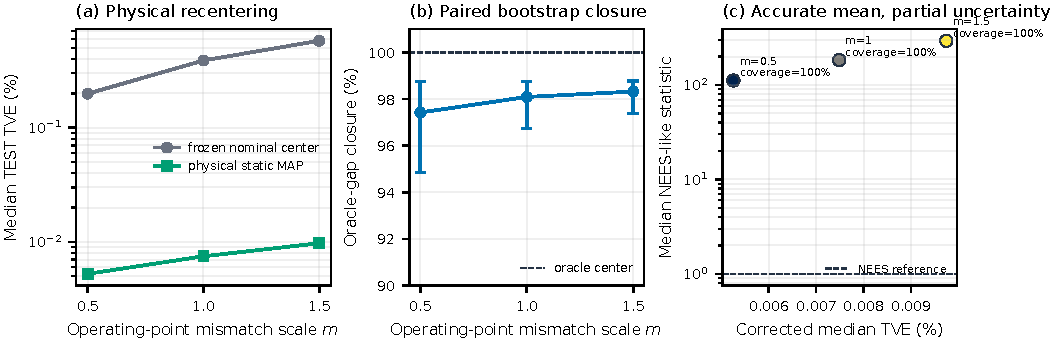
\includegraphics[width=\textwidth]{figures/generated/adequacy_adaptation.pdf}
\caption{Physical recentering repairs much of the tested point-estimate error while the joint uncertainty diagnostic remains inadequate.}\label{fig:supp-narrative-recenter}\end{figure*}

\subsection{Batch Source Resolution}
The historical implementation has an effective cardinality prior different
from its originally declared prior because of a single-source normalization
factor. The archived outcomes below are preserved, not corrected-prior
results or calibrated physical limits. The detailed qualification follows
in Section~\ref{sec:narrative-information} of this supplement.
The implemented batch estimator retains GH31 amplitude integration, W2 covariance, a fixed operating point and known onset/family. It evaluates the complete zero-, one- and two-source catalog; it does not supply the causal R11 decisions.
\begin{table*}[t]
\caption{Fresh prospective 137-hypothesis confirmation. The bank contains $H_0$, 16 single-source hypotheses, and all 120 two-source supports. Repeated noise realizations are decisions, not independent physical trajectories. Top-$k$ is exact support recovery and is undefined for $H_0$ and single-source rows in this exported support table.}
\label{tab:global137-results}
\centering
\footnotesize
\begin{tabular}{lrrrrrr}
\toprule
Regime & Physical trajectories & Decisions & Cardinality (\%) & Top-1 (\%) & Top-3 (\%) & Mean $p(K=2)$ \\
\midrule
No event & --- & 100 & 100.0 & --- & --- & 0.000 \\
Single source & 128 & 384 & 93.8 & --- & --- & 0.051 \\
Weak--weak pair & 1920 & 5760 & 37.4 & 24.4 & 59.8 & 0.427 \\
Weak--strong pair & 480 & 1440 & 77.6 & 66.2 & 95.8 & 0.808 \\
Moderate pair & 480 & 1440 & 99.7 & 98.8 & 100.0 & 0.996 \\
Finite pair & 480 & 1440 & 100.0 & 100.0 & 100.0 & 1.000 \\
\bottomrule
\end{tabular}
\end{table*}

\begin{figure*}[t]\centering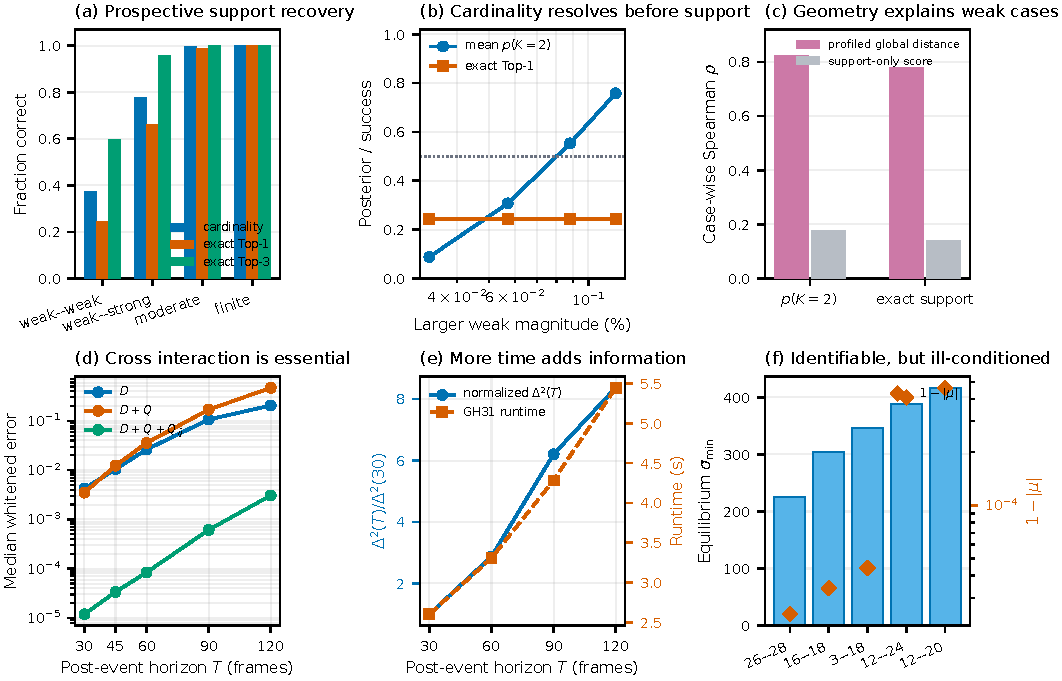
\includegraphics[width=\textwidth]{figures/generated/multi_event_evidence.pdf}
\caption{Expanded source-resolution study. Prospective recovery, retrospective profiled geometry and the longer-horizon diagnostic have distinct roles; the latter panels do not replace a new prospective test.}\label{fig:multi-event-evidence}\end{figure*}

\subsection{What the Reference Estimator Still Does Not Claim}
The historical supervised bank spans \LegacyEventTrajectories{} ANDES trajectories, with detection F1 \LegacyEventDetectionFOne{} and physical Top-1 \LegacyPhysicalTopOne{} on its own ordinary split. Its held-source stress test gives \HeldSourceCorrect{}/\HeldSourceDecisions{} exact decisions. These are different populations from H04/C01, so their scores cannot be subtracted to claim an improvement of the hackathon leaderboard. The unrestricted joint state/event/integrity estimator and learned discrepancy layer remain proposals. The pre-revision manuscript and its complete original main-text derivations are preserved in \texttt{archive/narrative\_before\_20261030/}.
\FloatBarrier
